\subsection{Impedance and Efficiency}

\begin{frame}{Impedance and Efficiency}
    \vspace{-6mm}
    \begin{columns}
        \column{0.4\textwidth}
        \begin{itemize}
            \item Impedance
        \end{itemize}
        \begin{equation*}
            R_r = \dfrac{2P}{I^2} = \dfrac{2\pi}{3} \eta \left( \dfrac{L}{\lambda} \right)^2.
        \end{equation*}
        \vspace{-3mm}
        \begin{itemize}
            \item Efficiency
        \end{itemize}
        \begin{equation*}
            e_r = \dfrac{P_r}{P_{in}} = \dfrac{R_r}{R_r+R_o}.
        \end{equation*}
        \vspace{-6mm}
        \begin{figure}
            \centering
            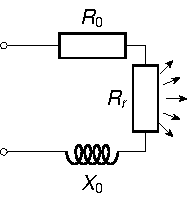
\includegraphics[width=0.6\textwidth]{Figures/Antenna_circuit.pdf}
            \caption{Antenna equivalent circuit.}
            \label{fig:Antenna_circuit}
        \end{figure}
        
        \column{0.6\textwidth}
        \begin{itemize}
            \item  Ohmic resistance for an antenna
        \end{itemize}
        \vspace{-3mm}
        \begin{figure}
            \centering
            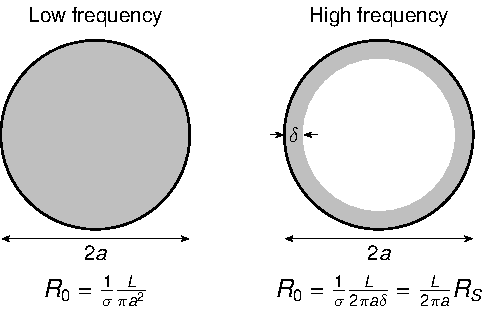
\includegraphics[width=\textwidth]{Figures/Skin_effect.pdf}
            \caption{Skin effect in high frequency.}
            \label{fig:Skin_effect}
        \end{figure}
        where \(\delta = \sqrt{2/ \omega \mu \sigma}\), \( R_S = \sqrt{\omega \mu / 2 \sigma }\).        
    \end{columns}
\end{frame}